\documentclass{standalone}
\usepackage{tikz}
\usepackage{ctex,siunitx}
\setCJKmainfont{Noto Serif CJK SC}
\usepackage{tkz-euclide}
\usepackage{amsmath}
\usepackage{wasysym}
\usetikzlibrary{patterns, calc}
\usetikzlibrary {decorations.pathmorphing, decorations.pathreplacing, decorations.shapes,}
\begin{document}
\small
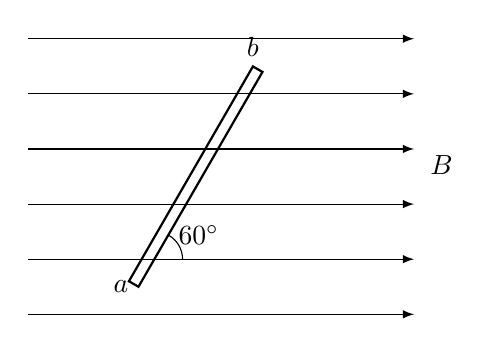
\begin{tikzpicture}[>=latex,scale=0.7]
  \foreach \x in {-.5,.5,...,4.5}
  {
     \draw [->](-2,\x)--(5,\x);
  }
  \draw [rotate=60, thick](0,0)node [left]{$a$} rectangle (4.5,.2)node [above]{$b$};
  \node at  (5.5,2.2){$B$};
  \draw (.8,.5) arc (0:60:.5) node[right]{$60^{\circ}$};
\end{tikzpicture}
\end{document}